\chapter{Invariant polynomial functions and covariants}


In this chapter $k$ is an infinite field. We also fix a finite-dimensional $k$-vector space $V$ with basis $(v_1, \ldots, v_n)$.


\begin{defi}
 By $\mc{P}(V)$ we denote set of polynomial functions $V \to k$, i.e. $f \in \mc{P}(V)$ if and only if $f : V \to k$ and there is some $p \in k[X_1, \ldots, X_n]$ such that
 \[
  f\left( \sum_{i=1}^n \lambda_i v_i \right) = p(\lambda_1, \ldots, \lambda_n)
 \]
 for all $\lambda_1, \ldots, \lambda_n \in k$.
\end{defi}


This definition does not depend on the chosen basis. If $(w_1, \ldots, w_n)$ is another basis of $V$ with $w_i = \sum_{j=1}^n a_{ij} v_j$ for $i=1,\ldots,n$ then
\begin{align*}
 f\left( \sum_{i=1}^n \lambda_i w_i \right)
 &= f\left( \sum_{i,j=1}^n \lambda_i a_{ij} v_j \right)
 = p\left( \sum_{i=1}^n \lambda_i a_{i1}, \ldots, \sum_{i=1}^n \lambda_{i} a_{in} \right)\\
 &= p'(\lambda_1, \ldots, \lambda_n)
\end{align*}
for some $p' \in k[X_1, \ldots, X_n]$. So if $f : V \to k$ is a polynomial in $(v_1, \ldots, v_n)$ then also in $(w_1, \ldots, w_n)$.


\begin{rem}
 If a group $G$ acts linearly on $V$ then it acts linearly on $\mc{P}(V)$ by $(g.f)(v) = f\left(g^{-1}.v\right)$.
\end{rem}


\begin{lem}
 There is an isomorphism of rings, even $k$-algebras
 \[
  \mc{P} \xlongrightarrow{\sim} k[X_1, \ldots, X_n]
 \]
 where $n = \dim V$.
\end{lem}
\begin{proof}
 For $1 \leq j \leq n$ define the $j$-th coordinate function (with respect to the chosen basis) as
 \[
  \varphi_j : V \to k, \sum_{i=1}^n \lambda_i v_i \mapsto \lambda_j.
 \]
 By the universal property of the polynomial ring the assignment $X_j \to \varphi_j$ extends to a ring homomorphism
 \[
  \Phi: k[X_1, \ldots, X_n] \to \mc{P}(V), p \mapsto \Phi(p)
 \]
 where
 \[
  \Phi(p)\left(\sum_{i=1}^n \lambda_i v_i\right) = p(\lambda_1, \ldots, \lambda_n).
 \]
 Is it clear that $\Phi$ is surjective. It is left as an exercise to the reader to check that $\Phi$ is injective.
\end{proof}


\begin{lem}\leavevmode
 \begin{enumerate}[a)]
  \item
   Assume $p \in k[X_1, \ldots, X_n]$ with $p(\lambda_1, \ldots, \lambda_n) = 0$ for all $(\lambda_1,\ldots,\lambda_n) \in k^n$. Then $p = 0$.
  \item
   The polynomial functions $\varphi_1, \ldots, \varphi_n \in \mc{P}(V)$ are algebraically independent over $k$, i.e. if $f(\varphi_1, \ldots, \varphi_n) = 0$ for some polynomial $f$ (over $k$) then $f = 0$.
 \end{enumerate}
\end{lem}
\begin{proof}\leavevmode
 \begin{enumerate}[a)]
  \item
   We show this by induction over $n$.
   
   ($n = 1$) Let $p \in k[X_1]$ with $p(\lambda_1) = 0$ for all $\lambda_1 \in k$. Since $k$ is infinite $p$ has infinitely many zeroes. Therefore $p = 0$.
   
   ($n \geq 2$) Assume the claim holds for $n-1$ and $1$. Consider $p \in k[X_1, \ldots, X_n]$ with $p(\lambda_1, \ldots, \lambda_n) = 0$ for all $(\lambda_1, \ldots, \lambda_n) \in k^n$. We write $p$ as
   \[
    p = \sum_{i \in \N} f_i(X_1, \ldots, X_{n-1}) X_n^i
   \]
   with $f_i \in k[X_1, \ldots, X_{n-1}]$ for all $i \in \N$ and $f_i = 0$ for all but finitely many $i \in \N$. Let $(\lambda_1, \ldots, \lambda_{n-1}) \in k^{n-1}$ be fixed but arbitrary. For all $\lambda_n \in k$ we have
   \[
    0 = p(\lambda_1, \ldots, \lambda_n) = \sum_{i \in \N} f_i(\lambda_1, \ldots, \lambda_{n-1}) \lambda_n^i
   \]
   By induction hypothesis we find that $f_i(\lambda_1, \ldots, \lambda_{n-1}) = 0$ for all $i \in \N$. Because $(\lambda_1, \ldots, \lambda_{n-1})$ is fixed but arbitrary we can use the induction hypothesis to get that $f_i = 0$ for all $i \in \N$. So $p = 0$.
  \item
   Assume $f(\varphi_1, \ldots, \varphi_n) = 0$. Then
   \[
    0 = f(\varphi_1, \ldots, \varphi_n)\left(\sum_{i=1}^n \lambda_i v_i\right) = f(\lambda_1, \ldots, \lambda_n)
   \]
   for all $(\lambda_1, \ldots, \lambda_n) \in k^n$. Therefore $f = 0$ by part a). \qedhere
 \end{enumerate}
\end{proof}

\begin{warn}
 The assumption that $k$ is infinite is necessary. If, for example, $p = X^2+X \in \F_2[X]$, then $p(0) = p(1) = 0$, so $p(\lambda)=0$ for all $\lambda \in k$, but $p \neq 0$.
\end{warn}


\begin{cor}
 The map $\Phi : k[X_1, \ldots, X_n] \to \mc{P}(V), X_j \mapsto \varphi_j$ is injective.
\end{cor}


Together with the exercise sheet we find that
\[
 \Phi : k[X_1, \ldots, X_n] \to \mc{P}(V), X_j \to \varphi_j
\]
is an isomorphism of $k$-algebras.


\begin{defi}
 $f \in \mc{P}(V)$ is homogeneous of degree $d \in \Z$ if $f(\lambda y) = \lambda^d f(y)$ for all $\lambda \in k, y \in V$. By definition the zero polynomial $f=0$ is homogeneous of degree $d$ for any $d \in \Z$. For $d \in \Z$ we set
 \[
  \mc{P}(V)_d := \{f \in \mc{P}(V) : f \text{ is homogeneous of degree } d\}.
 \]
\end{defi}


\begin{lem}\leavevmode
 \begin{enumerate}[a)]
  \item
   $\mc{P}(V)_d$ is a $k$-vector space for all $d \in \Z$ (via pointwise addition and scalar multiplication).
  \item
   If $f \in \mc{P}(V)_i$ and $g \in \mc{P}(V)_j$  then $fg \in \mc{P}(V)_{i+j}$, where the multiplication is given by pointwise multiplication.
 \end{enumerate}
\end{lem}
\begin{proof}\leavevmode
 \begin{enumerate}[a)]
  \item For $f_1, f_2 \in \mc{P}(V)_d$ we have
  \begin{align*}
   (f_1+f_2)(\lambda v)
   &= f_1(\lambda v) + f_2(\lambda v)
   = \lambda^d f_1(v) + \lambda^d f_2(v) \\
   &= \lambda^d (f_1(v) + f_2(v))
   = \lambda^d (f_1 + f_2)(v)
  \end{align*}
  for all $\lambda \in k, v \in V$, so $f_1 + f_2 \in \mc{P}(V)_d$. If $f \in \mc{P}(V)$ and $\mu \in k$ then
  \[
   (\mu f)(\lambda v) = \mu f(\lambda v) = \lambda^d \mu f(v) = \lambda^d (\mu f)(v),
  \]
  so $\mu f \in \mc{P}(V)_d$.
  \item
  For all $\lambda \in k$ we have for all $v \in V$
  \[
   fg(\lambda v)
   = f(\lambda v) g(\lambda v)
   = \left(\lambda^i f(v)\right)\left(\lambda^j g(v)\right)
   = \lambda^{i+j} f(v) g(v)
   = \lambda^{i+j} (fg)(v),
  \]
  and therefore $fg \in \mc{P}(V)_{i+j}$. \qedhere
 \end{enumerate}
\end{proof}


\begin{defi}
 A $k$-Algebra $A$ is called graded (or more precisely $\Z$-graded) if there is a decomposition $A = \bigoplus_{d \in \Z} A_d$ into vector subspaces $A_d$ sucht that $A_i A_j \subseteq A_{i+j}$ for all $i,j \in \Z$.
 
 A ring $R$ is called graded if there is a decomposition $R = \bigoplus_{d \in \Z} R_d$ into $\Z$-modules such that $R_i R_j \subseteq R_{i+j}$ for all $i,j \in \Z$.
 
 We call $A_d$, resp. $R_d$, the homogeneous part of degree $d$.
\end{defi}

\begin{rem}
 If $A$ is a $k$-Algebra with $1$, then $A$ is a graded $k$-Algebra if and only if $A$ is a graded ring such that $k1 \subseteq A_0$.
\end{rem}
\begin{proof}
 ($\Rightarrow$) Because $A$ is a graded $k$-Algebra there exists a decomposition $A = \bigoplus_{d \in \Z} A_d$ into vector subspaces such that $A_i A_j \subseteq A_{i+j}$ for all $i,j \in \Z$. It is clear that this is also a decomposition into $\Z$-modules.
 
 We first notice that $1 \in A_0$: Because $1 \in A = \bigoplus_{d \in \Z} A_d$ there exist unique $e_i \in A_i$ with $1 = \sum_{i \in \Z} e_i$ with $e_i = 0$ for all but finitely many $i$. For every $j \in \Z$ and $a \in A_j$ we have
 \[
  a = a \cdot 1 = a \cdot \sum_{i \in \Z} e_i = \sum_{i \in \Z} \underbrace{a e_i}_{\in A_{i+j}}.
 \]
 Because the sum $A = \bigoplus_{d \in \Z} A_d$ is direct we find that $a = a e_0$. Because $A = \bigoplus_{d \in \Z} A_d}$ we find that $a e_0 = a$ for all $a \in A$. This shows that $1 = e_0$ and therefore $1 \in A_0$. Because $A_0$ is a vector subspace it follows that $\lambda 1 \in A_0$ for all $\lambda \in k$.
 
 ($\Leftarrow$) Suppose $A = \bigoplus_{d \in \Z} A_d$ such that $A_d$ is a $\Z$-module for all $d \in \Z$ and $A_i A_j \subseteq A_{i+j}$ for all $i,j \in \Z$. We only need to check that $A_d$ is closed under scalar multiplication. This holds because
 \[
  \lambda A_d = \lambda 1 A_d \subseteq A_0 A_d \subseteq A_d \text{ for all } \lambda \in k
 \]
 for all $d \in \Z$.
\end{proof}


\begin{expls}\leavevmode
 \begin{enumerate}[a)]
  \item
  Let $A$ be a $K$-algebra. Then $A$ is a graded $k$-Algebra via $A_0 = A$ and $A_d = 0$ für $d \neq 0$.
  
  \item
  Let $k$ be a field (or a ring). $k[X_1, \ldots, X_n]$ is a graded $k$-algebra (or a graded ring) by setting
  \[
   A_d :=
   \begin{cases}
    \vspan_k(\{X_1^{\alpha_1} \cdots X_n^{\alpha_n} : \sum_{i=1}^n a_i = d\}) & \text{if } d \geq 0, \\
    0                                                                         & \text{otherwise}.
   \end{cases}
  \]
  By definition $A_d$ is a $k$-vector space (or $\Z$-module). Since the monomials form a $k$-Basis of $k[X_1, \ldots, X_n]$ we have $A = \bigoplus_{d \geq 0} A_d = \bigoplus_{d \in \Z} A_d$. Since
  \[
   \left( X^{\alpha_1} \cdots X^{\alpha_n} \right) \left( X^{\beta_1} \cdots X^{\beta_n} \right)
   = X_1^{\alpha_1+\beta_1} \cdots X_n^{\alpha_n+\beta_n}
  \]
  we find that for monomials $f \in A_i$ and $g \in A_j$ $fg \in A_{i+j}$. By extending this linearly we get that $A_i A_j \subseteq A_{i+j}$ for all $i,j \in \Z$.
  
  \item
  $\mc{P}(V)$ inherts a grading from $k[X_1, \ldots, X_n] =: A$ via the isomorphism $\Phi$. Since
  \[
   (\lambda X_1)^{\alpha_1} \cdots (\lambda X_n)^{\alpha_n}
   = \lambda^{\sum_{i=1}^n \alpha_i} X_1^{\alpha_1} \cdots X_n^{\alpha_n}
  \]
  we obtain that a monomial of degree $d$ (i.e. $p \in A_d$) corresponds to a polynomial function $\Phi(p) \in \mc{P}(V)$ which is homogeneous of degree $d$. Therefore $\mc{P}(V)$ is a graded algebra via
  \[
   \mc{P}(V) = \bigoplus_{d \in \Z} \mc{P}(V)_d.
  \]
  
  \item
  $T(V) := k \oplus \bigoplus_{d \geq 1} V^{\otimes d}$ is an algebra by extending
  \[
   (v_{i_1} \otimes \ldots \otimes v_{i_k}) \cdot (v_{j_1} \otimes \ldots \otimes v_{j_n})
   = v_{i_1} \otimes \ldots \otimes v_{i_k} \otimes v_{j_1} \otimes \ldots \otimes v_{j_n}
  \]
  with $v_{i_1}, \ldots, v_{i_k}, v_{j_1}, \ldots, v_{j_n} \in V$ linearly. (We leave it as an exercise to check that this is indeed a $k$-algebra.) $T(V)$ is a graded algebra via
  \[
   T(V) = \bigoplus_{d \in \Z} T(V)_d,
  \]
  where
  \[
   T(V)_d =
   \begin{cases}
    V^{\otimes d} & \text{if } d > 0, \\
    k             & \text{if } d = 0, \\
    0             & \text{if } d < 0.
   \end{cases}
  \]
 \end{enumerate}
\end{expls}


\begin{defi}
 A $k$-algebra $A$ is filtered if there exists a (potentially infinite) sequence
 \[
  0 = F_{-1}(A) \subseteq F_0(A) \subseteq F_1(A) \subseteq F_2(A) \subseteq \ldots \subseteq A
 \]
 of $k$-vector subspaces $F_i(A)$ such that
 \begin{enumerate}[1)]
  \item $\bigcup_i F_i(A) = A$ and
  \item $F_i(A) F_j(A) \subseteq F_{i+j}(A)$ for all $i,j$.
 \end{enumerate}
 This sequence is called a filtration of $A$.
\end{defi}


\begin{defi}
 If $A$ is a filtered algebra and
 \[
  0 = F_{-1}(A) \subseteq F_0(A) \subseteq F_1(A) \subseteq F_2(A) \subseteq \ldots \subseteq A
 \]
 a filtration of $A$, then define for all $i \geq 0$
 \[
  (\gr_\mc{F}A)_i := F_i(A)/F_{i-1}(A)
 \]
 and
 \[
  \gr_\mc{F}(A) := \bigoplus_{i \geq 0} (\gr_\mc{F}A)_i.
 \]
 $\gr_\mc{F}(A)$ is the associated graded algebra to the filtered algebra $A$
\end{defi}



\begin{lem}
 $\gr_\mc{F}(A) = \bigoplus_{i \geq 0} (\gr_\mc{F}A)_i$ is a graded algebra with the multiplication indexed from the multiplication of $A$, i.e.
 \[
  ( a + F_{i-1}(A) )( b + F_{j-1}(A) ) = ab + F_{i+j-1}(A).
 \]
\end{lem}
\begin{proof}
 The multiplication is well defined: Let $a \in F_i(A), b \in F_j(A)$. Note that we have
 \begin{align*}
  F_{i-1}(A)F_j(A) &\subseteq F_{i+j-1}(A), \\
  F_i(A) F_{j-1}(A) &\subseteq F_{i+j-1}(A) \text{ and } \\
  F_{i-i}(A)F_{j-1}(A) &\subseteq F_{i+j-2}(A) \subseteq F_{i+j-1}(A).
 \end{align*}
 Because of this, we have for all $x_1 \in F_{i-1}(A)$ and $x_2 \in F_{j-1}(A)$ that
 \[
  (a + x_1)(b + x_2) = a b + x
 \]
 for some $x \in F_{i+j-1}(A)$. So we get a well-defined multiplication
 \begin{align*}
  (\gr_\mc{F} A) \times (\gr_\mc{F} A) &\to \gr_\mc{F} A, \\
  (a + F_{i-1}, b + F_{j-i}) &\mapsto ab + F_{i+j-1}.
 \end{align*}
 It now easily follows that $\gr_\mc{F} A$ is an associative algebra.
 
 It is clear, that $(\gr_\mc{F} A)_i$ is a $k$-vector subspace of $\gr_\mc{F} A$, and by the definition of the multiplication we have
 \[
  (\gr_\mc{F} A)_i (\gr_\mc{F} A)_j \subseteq (\gr_\mc{F} A)_{i+j} \text{ for all } i,j \geq 0.
 \]
 This shows that $\gr_\mc{F} A$ is a graded algebra.
\end{proof}


\begin{lem}
 Let $A = \bigoplus_{d \in \Z} A_d$ be a graded $k$-algebra with $A_d = 0$ for all $d < 0$. Then
 \[
  F_i(A) := \bigoplus_{d \leq i} A_d \text{ for all } i \geq -1
 \]
 defines a filtration on $A$.
\end{lem}
\begin{proof}
 $F_i(A)$ is a vector subspace for all $i \geq -1$, because $A_d$ is a vector subspace for all $d \in \Z$. It is also clear that $F_{-1}(A) = 0$ and $F_i(A) \subseteq F_{i+1}(A)$ for all $i \geq -1$. Since $A = \bigoplus_{d \geq 0} A_d$ we have that $A = \bigcup_{i \geq -1} F_i(A)$. We also have
 \begin{align*}
  F_i(A) F_j(A)
  &= \left( \bigoplus_{d \leq i} A_d \right) \left( \bigoplus_{d \leq j} A_d \right)
  \subseteq \sum_{\substack{d_1 \leq i \\ d_2 \leq j}} A_{d_1 + d_2}
  \subseteq \bigoplus_{d \leq i+j} A_d \\
  &= F_{i+j}(A).
 \end{align*}
\end{proof}


\begin{expl}
 Consider $k[X]$ for some field $k$. Then the multiplication with $X$ defines an element $X \in \End_k(k[X])$. Let $\partial = \partial/\partial x \in \End_k(k[X])$ be the (formal) derivative with respect to $X$.
 
 Consider the subalgebra $\mc{A}_1$ of $\End_k(k[X])$ generated by $X$ and $\partial$. Then $\mc{A}_1 \cong k\gen{X,\partial}/\mc{I}$ where $\mc{I} \subseteq k \gen{X,\partial}$ is the two sided ideal generated by the element $\partial X - X \partial - 1$. The images of the monomials $X^\alpha \partial^\beta$, $\alpha, \beta \in \N$ under this isomorphism form a $k$-basis of $\mc{A}_1$. We can then define
 \[
  F_i(\mc{A}_1) := \vspan_k(\{\text{images of $X^\alpha \partial^\beta$ where $\alpha+\beta \leq i$}) \text{ for all } i \geq -1.
 \]
 This gives us a filtration on $\mc{A}_1$. (We leave the proof of this claims as an exercise to the reader. It will also appear on the exercise sheets.)
\end{expl}

\begin{defi}
Let $G$ be a group, $k$ any field and $V,W$ representations of $G$. A map $f : V \to W$ is called a morphism of $G$-spaces or morphism  of representations of $G$ if $f$ is $k$-linear and $G$-equivariant. An isomorphism of representations is an morphism of representations which is also invertible as a $k$-linear map. We call $V$ and $W$ isomorphic (as representations of $G$), denoted by $V \cong W$, if there exists an isomorphism of representations between $V$ and $W$. We denote
\[
 \Hom_G(V,W) = \{f : V \to W \,|\, f \text{ is a morphism of representations}\}.
\]
\end{defi}


\begin{rem}
 If $f : V \to W$ is an isomorphism of representations, then its linear inverse $f^{-1}$ is again a morphism of representations, because $f^{-1}$ is linear by definition and it is $G$-equivariant, because for all $g \in G, v \in V$
 \[
  f\left(f^{-1}(g.v)\right) = g.v = g.f\left(f^{-1}(v)\right) = f\left(g.f^{-1}(v)\right)
 \]
 and $f$ is bijective (and therefore injective).
\end{rem}


\begin{rem}
 If $V$ and $W$ are representations of $G$ then $\Hom_G(V,W)$ is a $k$-vector space via pointwise addition und scalar multiplication. (This will be on one of the exercise sheets.)
\end{rem}


\begin{lem}\label{lem: composition of morphisms of representations}
 Let $G$ be a group.
 \begin{enumerate}[a)]
  \item
  $\id_V : V \to V$ is a morphism of representations for any representation $V$ of $G$.
  \item
  If $f : V \to W$  and $g : W \to Z$ are morphism of representations of $G$, then $g \circ f : V \to Z$ is a morphism of representations.
 \end{enumerate}
\end{lem}
\begin{proof}
 Part a) is trivial. It is also clear that $g \circ f$ is $k$-linear and $G$-equivariant (see the proof in chapter I for $G$-sets).
\end{proof}


\begin{lem}\label{lem: ker and im subrepresentations}
 Let $V,W$ be representations of a group $G$, $f \in \Hom_G(V,W)$. Then $\ker f$ is a subrepresentation of $V$ and $\im f$ is a subrepresentation of $W$.
\end{lem}
\begin{proof}
 Since $f$ is linear, $\ker f$ is a vector subspace of $V$ and $\im f$ is a vector subspace of $W$.
 
 Let $x \in \ker f$. Then $f(g.x) = g.f(x) = g.0 = 0$ for all $g \in G$, because $G$ acts linear. So $g.x \in \ker f$ for all $g \in G, x \in \ker f$.
 
 Let $y = f(x) \in \im f$. Then $g.y = g.f(x) = f(g.x) \in \im f$ for all $g \in G$.
\end{proof}


\begin{lem}[Schur’s Lemma]
 Let $k$ be a field, $G$ a group, $V$ and $W$ irreducible representations of $G$.
 \begin{enumerate}[a)]
  \item
  We have $\Hom_G(V,W) = 0$ if $V \not\cong W$ and $\Hom_G(V,W) \not\cong 0$ if $V \cong W$, and every non zero morphism is an isomorphism.
  \item
  $\Hom_G(V,V)$ is a divison ring / skew field (i.e. we have $1 \neq 0$ and every non zero endomorphism is invertible).
  \item
  In the special case that $k$ is algebraically closed (e.g. $k = \C$) and $V$ and $W$ are both finite dimensional we have that
  \[
   \Hom_G(V,W) \cong
   \begin{cases}
    k & \text{if } V \cong W, \\
    0 & \text{if } V \not\cong W,
   \end{cases}
  \]
  as vector spaces.
 \end{enumerate}
\end{lem}
\begin{proof}
 \begin{enumerate}[a)]
  \item 
  Assume $0 \neq f \in \Hom_G(V,W)$. Then by Lemma \ref{lem: ker and im subrepresentations} $\ker f$ and $\im f$ are subrepresentations of $V$, resp. $W$. Since $V$ and $W$ are irreducible we have that
  \[
   \ker f = 0 \text{ or } \ker f = V \quad \text{and} \quad \im f = 0 \text{ or } \im f = W.
  \]
  Since $f \neq 0$ we have $\ker f \neq V$ and $\im f \neq 0$. So $\ker f = 0$ and $\im f = W$.
  \item
  It is clear that $V \cong V$, so it follows from a).
  \item
  Assume $\alpha, \beta \in \Hom_G(V,W)$ where $V \cong W$ and $\alpha \neq 0$. It is enough to show that there exists some $\lambda \in k$ such that $\beta = \lambda \alpha$. Consider the morphism $\alpha^{-1} \beta \in \Hom_G(V,W)$ (this is well defined since we know from a) that $\alpha$ is invertible and $\alpha^{-1}$ is again a morphism of representations by the previous Remark, hence $\alpha^{-1} \beta \in \Hom_G(V,W)$ by lemma \ref{lem: composition of morphisms of representations}).
  
  Because $k$ is algebraically closed $\alpha^{-1} \beta$ has some eigenvalue $\lambda \in k$. By \mbox{lemma \ref{lem: ker and im subrepresentations}}
  \[
   K := \ker(\alpha^{-1} \beta - \lambda \id_V)
  \]
  is a subrepresentation of $V$. Since $V$ is irreducible and $K \neq 0$ (because $\lambda$ is an eigenvalue of $\alpha^{-1} \beta$) we have $K = V$. So $\alpha^{-1} \beta = \lambda \id_V$ and therefore $\beta = \lambda \alpha$. \qedhere
 \end{enumerate}
\end{proof}


\begin{rem}
 Assume $k$ is an algebraically closed field and $V$ a finite dimensional irreducible representation of some group $G$. Then
 \[
  \End_G(V \oplus \ldots \oplus V)
  := \Hom_G(V \oplus \ldots \oplus V, V \oplus \ldots \oplus V)
  \cong \Mat(n \times n, k)
 \]
 is an isomorphism of rings by Schur’s lemma part c).
 
 More general: Let $V_1, \ldots, V_r$ be pairwise non-isomorphic irreducible finite dimensioal representations of some group $G$ and $W_i := V_i^{n_i}$. Then
 \begin{align*}
  \End_G(W_1 \oplus \ldots \oplus W_r)
  &= \End(V_1^{n_1} \oplus \ldots \oplus V_n^{n_r}) \\
  &\cong \End(V_1^{n_1}) \oplus \ldots \oplus \End(V_r^{n_r}) \\
  &\cong \Mat(n_1 \times n_1, k) \oplus \ldots \oplus \Mat(n_r \times n_r, k)
 \end{align*}
 as rings.
\end{rem}


\begin{defi}
 Let $G$ be a group. A representation $V$ of $G$ (over a field $k$) is completely reducible if
 \[
  V \cong V_1 \oplus \ldots \oplus V_r
 \]
 for some irreducible representations $V_1, \ldots, V_r$.
\end{defi}


\begin{rem}
 Not every representation is completely reducible, even if $k$ is algebraically closed. Consider, for example,
 \[
  G := \left\{\vect{a & b \\ 0 & c} \,\middle|\, a,b,c \in \C \text{ and } a,c \neq 0\right\}
  \subseteq \GL_2(\C)
 \]
 and the natural representation of $G$ on $\C^2$. We saw earlier that $U := \vspan(e_1)$ gives a subrepresentation and it’s the only $1$-dimensional subrepresentation. So the representation is not irreducible, but at the same time not isomorphic to a direct sum of irreducible representations.
\end{rem}


\begin{thrm}[Maschke’s theorem]
 Let $G$ be a finite group and $k$ a field such that $\kchar k \nmid |G|$ (in particular $\kchar k = 0$ is allowed). Then any finite dimensional representation of $G$ over $k$ is completely reducible.
\end{thrm}
\begin{proof}
 It is enough to show that every subrepresentation $U$ of $V$ has a complement $W$ which is again a subrepresentation, i.e. $V = U \oplus W$ as representations.
 
 Given our subrepresentation $U$ choose a complement $W$ as a vector space. Then $V = U \oplus W$ as vector spaces. Let $p : V \to U$ be the orthogonal projection onto $U$. ($p$ is not necessarily $G$-equivariant but only a linear map.) We know that $\im p = U$. We define $\hat{p} : V \to U$ as
 \[
  \hat{p}(v) := \frac{1}{|G|} \sum_{g \in G} g^{-1}.p(g.v).
 \]

This is well defined since $|G| < \infty$ and $1/|G|$ is defined, because $\kchar k \nmid |G|$. Note that $\im \hat{p} \subseteq U$, since $p(g.v) \in U$ and $U$ is a subrepresentation, hence $g^{-1}.p(g.v) \in U$ for all $g \in G, v \in V$.

It is clear that $\hat{p}(u) = u$ for all $u \in U$ because
\[
 \hat{p}(u)
 = \frac{1}{|G|} \sum_{g \in G} g^{-1}.p(g.u)
 = \frac{1}{|G|} \sum_{g \in G} g^{-1}.g.u
 = \frac{1}{|G|} \sum_{g \in G} u
 = u.
\]
$\hat{p}$ is $G$-equivariant because for all $h \in G$ and $v \in V$
\begin{align*}
 \hat{p}(h.v)
 &= \frac{1}{|G|} \sum_{g \in G} g^{-1}.p(gh.v)
 = \frac{1}{|G|} \sum_{g \in G} h.h^{-1}.g^{-1}.p(g.h.v) \\
 &= \frac{1}{|G|} \sum_{\bar{g} \in G} h.\bar{g}^{-1}.p(\bar{g}.v)
 = h.\hat{p}(v).
\end{align*}
Altogether we have
\begin{center}
 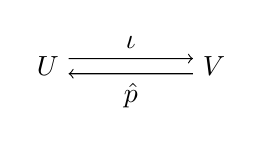
\begin{tikzpicture}[node distance = 6em, auto]
  \node (U) {$U$};
  \node (V) [right of = U] {$V$};
  \draw[->] (U.20) to node {$\iota$}(V.160);
  \draw[->] (V.200) to node {$\hat{p}$} (U.340);
 \end{tikzpicture}
\end{center}
where both maps are $G$-equivariant and $\hat{p} \iota = \id_U$. So the projection $\hat{p}$ splits and we obtain $V \cong U \oplus \ker \hat{p}$. Because $\hat{p}$ is $G$-equivariant $\ker \hat{p}$ is a subrepresentation of $V$. So $U$ has a complement which is again a representation.
\end{proof}

\begin{warn}
 The theorem is wrong in general if $\kchar k \mid |G|$. (An example will be on the exercise sheet.)
\end{warn}

\begin{expl}
 In general it is hard to compute a decomposition using Maschke’s theorem in practice!
 
 Let $G = S_3$. Let $V = kG$ be viewed as a representation of $G$ via the left multiplication, i.e.
 \[
  h.\left(\sum_{g \in G} a_g g\right) = \sum_{g \in G} a_g hg.
 \]
 Let $k = \C$, hence Maschke’s theorem holds. We want to find a decomposition of $kG$. Recall that $S_3 = \gen{s,t}$ where $s = (1 \; 2)$ and $t = (2 \; 3)$. We claim that
 \[
  kG = V_{\text{triv}} \oplus V_{\text{sgn}} \oplus V_1 \oplus V_2
 \]
 where
 \begin{align*}
  V_{\text{triv}} &:= \vspan\left(\sum_{g \in G} g \right) = \vspan(e+s+t+st+ts+sts), \\
  V_{\text{sgn}} &:= \vspan\left(e-s-t+st+ts-sts\right), \\
  V_1 &:= \vspan\left(e+s-ts, t+ts-st-sts\right) \text{ and} \\
  V_2 &:= \vspan\left(s+st-sts,e+t-s-st\right).
 \end{align*}
 Note that $G$ acts trivially on $V_{\text{triv}}$ and by multiplication with $-1$ on $V_{\text{sgn}}$ , hence $V_{\text{triv}}$ and $V_{\text{sgn}}$ are subrepresentations. One can also check that $V_1$ and $V_2$ are irreducible subrepresentations which are isomorphic.
\end{expl}


\begin{expl}
 Let $n \geq 2$ and $G = S_n$. Let $k$ be any field and let $S_n$ act on $k^n$ by setting
 \[
  g.e_i = e_{g(i)}
 \]
 where $e_1, \ldots, e_n$ denotes the standard basis of $k^n$. Extending this linearly we get a representation of $G$ on $k^n$, i.e.
 \[
  g.(a_1, \ldots, a_n) = \left(a_{g^{-1}(1)}, \ldots, a_{g^{-1}(n)}\right).
 \]
 We can then set $V = k^n$ and extend the $G$-action on $V$ to be a $G$-action on $\mc{P}(V)$ by setting $(g.f)(v) = f(g^{-1}.v)$ for all $f \in \mc{P}(V), v \in V$. We can then ask ourselves how to describe $\mc{P}(V)$.
\end{expl}


\begin{defi}
 Let $k$ be a group and $W$ any $k$-vector space. Then $g.w = w$ for all $g \in G, w \in W$ defines a representation $W$ of $G$. This is called the trivial representation. For each fixed dimension there is (up to isomorphism) one trivial representation. Therefore we usually say \emph{the} trivial representation of $G$ (of dimension $\dim W$).
\end{defi}


\begin{lem}
 Let $\{e_1, \ldots, e_n\}$ denote the standard basis von $k^n$. $G = S_n$ acts linearly on $k^n$ as in the previous example.
 \begin{enumerate}[a)]
  \item
  The vector subspaces
  \begin{gather*}
   U_1 := \vspan\left( \sum_{i=1}^n e_i\right)
  \shortintertext{and}
   U_2 := \left\{ (\lambda_1, \ldots, \lambda_n) \in k^n \,\middle|\, \sum_{i=1}^n \lambda_i = 0 \right\}
  \end{gather*}
  are subrepresentations.
  \item
  $U_1$ is the trivial $1$-dimensional subrepresentation and
  \[
   \begin{cases}
    U_1 \cong U_2 & \text{if } n = 2, \kchar k = 2,\\
    U_1 \ncong U_2 & \text{otherwise}.
   \end{cases}
  \]
  \item
  In the second case $V$ is completely irreducible, in the first case it isn't.
 \end{enumerate}
\end{lem}
\begin{proof}
 \begin{enumerate}
  \item
  It is clear that $U_1$ and $U_2$ are vector subspaces. Since
  \[
   g.\left(\sum_{i=1}^n e_i\right)
   = \sum_{i=1}^n e_{g(i)}
   = \sum_{i=1}^n e_i
   \tag{$\ast$}
  \]
  we have $g.u \in U_1$ for all $g \in G, u \in U_1$, thus $U_1$ is a subrepresentation. Since
  \[
   g.(\lambda_1, \ldots, \lambda_n) = \left( \lambda_{g^{-1}(1)}, \ldots, \lambda_{g^{-1}(n)} \right)
  \]
  we have $g.u \in U_2$ for all $g \in G, u \in U_2$, thus $U_2$ is a subrepresentation.
  \item
  We have that $g.u = u$ for all $u \in U$ by ($\ast$).  If $n > 2$ then
  \[
   \dim U_1 = 1 \neq \dim U_2
  \]
  and thus $U_1 \ncong U_2$.
  
  If $n = 2$ and $S_2 = \{e,s\}$ then $s.(1,1) = (1,1)$ for the basis vector $(1,1)$ of $U_1$ and $s.(1,-1) = -(1,-1)$ for the basis vector $(1,-1)$ of $U_2$. So $U_2$ is not the trivial representation if $\kchar k \neq 2$, and thus $U_1 \ncong U_2$.  If $\kchar k = 2$ then $U_1 = U_2$ and in particular $U_1 \cong U_2$. 
  \item
  This part of the proof still needs to be typed. \qedhere
  %TODO: Beweis vervollständigen.
 \end{enumerate}
\end{proof}


\begin{rem}
 In the case of $n = 2$ the representation $U_2$ is called the sign representation.
 %TODO: Sign-Darstellung besser erklären.
\end{rem}


\begin{defi}
 Let $k$ be a field. $G := S_n$ acts linearly on $k[X_1, \ldots, X_n]$ by extending
 \[
  g.X^{\alpha_1} \cdots X_n^{\alpha_n} = X_{g(1)}^{\alpha_1} \cdots X_{g(n)}^{\alpha_n} \text{ for all } g \in G
 \]
 linearly. A polynomial $f \in k[X_1, \ldots, X_n]^{S_n}$ is called a symmetric polynomial (in $n$ variables).
\end{defi}


\begin{rem}
 For $k$ infinite and $V = k^n$ we have an isomorphism of representations
 \[
  \Phi : k[X_1, \ldots, X_n] \to \mc{P}(V), X_i \mapsto \varphi_i,
 \]
 where $G$ acts on $\mc{P}(V)$ via
 \[
  (g.f)(v) = f\left( g^{-1}.v \right) \text{ for all } g \in G, f \in \mc{P}(V), v \in V.
 \]
 We know that $\Phi$ is an isomorphism of $k$-vector spaces. It is $G$-equivariant, since for all $g \in G, p = X_1^{\alpha_1} \cdots X_n^{\alpha_n} \in k[X_1, \ldots, X_n], (\lambda_1, \ldots, \lambda_n) \in k^n = V$
 \begin{align*}
  \Phi(g.p)(v)
  &= \Phi\left( X_{g(1)}^{\alpha_1} \cdots X_{g(n)}^{\alpha_n} \right)(v)
  = \lambda_{g(1)}^{\alpha_1} \cdots \lambda_{g(n)}^{\alpha_n} \\
  &= \Phi(p)\left( g^{-1}.(\lambda_1, \ldots, \lambda_n) \right)
  = (g.\Phi(p))(\lambda_1, \ldots, \lambda_n).
 \end{align*}
\end{rem}

\begin{expl}
 In $k[X_1, X_2, X_3]$ we have the symmetric polynomials
 \begin{align*}
  p_2 &:= X_1^2 + X_2^2 + X_3^2, \\
  h_2 &:= X_1^2 + X_1 X_2 + X_1 X_3 + X_2^2 + X_2 X_3 + X_3^2, \\
  e_2 &:= X_1 X_2 + X_1 X_3 + X_2 X_3 \text{ and} \\
  m_{(4,4,2)} &:= X_1^4 X_2^2 X_3^2 + X_1^2 X_2^4 X_3^2 + X_1^2 X_2^2 X_3^4.
 \end{align*}
 More generally in $k[X_1, \ldots, X_n]$ we have the following symmmetric polynomials:

 The $r$-th power symmetric polynomial, also called the $r$-th power sum,
 \[
  p_r := p_r^{(n)} = X_1^r + \ldots + X_n^r,
 \]
 the $r$-th completely symmetric polynomial
 \[
  h_r := h_r^{(n)} = \sum_{|\alpha|=r} X_1^{\alpha_1} \cdots X_n^{\alpha_n}.
 \]
 and the $r$-th elementary symmetric polynomial
 \[
  e_r := e_r^{(n)} = \sum_{1 \leq i_1 < \ldots < i_r \leq n} X_{i_1} \cdots X_{i_r}
 \]
 We also set $e_0^{(n)} := 1$ and $e_r^{(n)} = 0$ for $r > n$.
\end{expl}









